\documentclass[fontsize=11pt, paper=a4, DIV=12]{scrartcl}

\usepackage{amsmath}
\usepackage{graphicx}
\graphicspath{ {./images/} }
\usepackage[center]{caption}
\usepackage{gensymb}
\usepackage{fancyhdr}
\usepackage{hyperref}
\hypersetup{
    colorlinks,
    citecolor=black,
    filecolor=black,
    linkcolor=black,
    urlcolor=black
}

\title{Microscope}
\date{14.11.2024}
\author{Leander Koufen, Sayann Travers, Livi Winker\\
Tutor: Sandeeta Thakur}

\pagestyle{fancy}
\fancyhf{}
\fancyhead[L]{Microscope}
\fancyhead[R]{\thepage}
\newcommand\numberthis{\addtocounter{equation}{1}\tag{\theequation}}

\begin{document}

\maketitle

\tableofcontents
\clearpage

\section{Preamble}
The first aim of this experiment is to construct a microscope and then to determine the magnification for three different tube lengths
and comparing the results with the theoretical expectation. After this the ocular is to be calibrated, to enable the measurement of the
distance between and the width of the wires of a wire grating.
Lastly the resolvable separation and the numerical aperture is to be calculated using the measured resolution limit.

\newpage

\section{Physical Principals}

The following physical basics are necessary for understanding the experiment:

\subsection{Lenses}

Light is defined as an electromagnetic wave. But for the purposes of this experiment it is to be interpreted as a ray 
that is being emitted by a light source, which can be broken or reflected. When parallel rays of light hit a convex lens they get broken 
in such a way that they gathers at the focal point F of said lense (see $\ref{A}$). G represents the height of hte object which is being 
viewed through the lense, g is the distance between the object and the lense. B is the image of the object and b similarly the distance between 
the lense and the image. 

\label{A}
\begin{figure}[h!]
    \centering
  \includegraphics[angle=270,scale=0.5]{Beam path of a concex lense.jpg}
  \caption{beam path of a convex lense}
  \end{figure}

The relationship between B and G or b and g is described in $\ref{1}$

\label{1}
\begin{align*}
    \frac{B}{G} & = \frac{b}{g} \tag{1}
\end{align*}

\subsection{Magnification}

b is the width of the eye and g is the distance between the object and the eye, which should be 

\begin{equation}
a_{0} = 25 cm 
\end{equation}

for maximum resolution. Magnification means that the image which reaches the back of the eye is enlarged through the use 
of an optical intrument. The proportion of B and G can be calcuated thus:

\label{2}
\begin{align*}
    \gamma & = \frac{tan(\alpha_{2})}{tan(\alpha_{1})} \tag{1}
\end{align*}


\label{B}
\begin{figure}[h!]
    \centering
  \includegraphics[angle=270,scale=0.5]{Effects of a lense on the eye (1).jpg}
  \caption{beam path of a ray of light through eye with (right) and without (left) lense}
  \end{figure}

A magnifying glass relies on the principle that when the object is placed between the focal point F and the convex lense a virtual 
image is created, which is further back and larger than the object. Since the image is virtual it cannot be projected onto a screen, 
but it has the effect of an enlarged real image being presented to the observer.
The magnification, based on the equation $\ref{2}$, can be calculated thus:

\label{3}
\begin{align*}
    \gamma_{magnifying} & = \frac{tan(\alpha-{2})}{tan(\alpha_{1})} \\
    & = \frac{G/f}{G/a_{0}} \\
    & = \frac{a_{0}}{f}      \tag{3}
\end{align*}

\subsection{Microscope}

\label{C}
\begin{figure}[h!]
    \centering
  \includegraphics[angle=270,scale=0.5]{Beam path microscope.jpg}
  \caption{beam path of ray of light through a microscope}
  \end{figure}

A microscope constitutes of two convex lenses: an objecte and the ocular. The obeject is placed  between the focal length and twice the 
focal length of the objective. This creates a real image between the objective and the ocular, which should be in betweem the ocular and 
its focal point $F_{ok}$. The real image $B_{Z}$ is then magnified following the same principle as that of the magnifying glass, which to
an enlarged image being presented to the viewer throgh the ocular.
In this case, the magnification of two lenses is calculated using the equation:

\label{4}
\begin{equation}
  \gamma_{mik} = \gamma_{ob} \cdot \gamma_{ok} \tag{4}
  \end{equation}

The theoretical magnification of the obejective can be calculated using the tube length t and the distance between the ocular and the viewers
eye ($a_{0}$).

\label{5}
\begin{equation}
  \gamma_{ob} = \frac{t}{f_{ob}} \tag{5}
  \end{equation}

Based on the equation $\ref{3}$ the calculation of the magnification of the ocular is apparent:

\label{3.1}
\begin{align*}
  \gamma_{ok} &= \frac{a_{0}}{g} \\
  &= \frac{a_0}{f_{ok}} \tag{3.1}
\end{align*}

For $\gamma_{ok}$ at the distance of $a_{0}$ ($\gamma_{ok}(a_{0})$) the equation $\ref{6}$ has to be taken into account:

\label{6}
\begin{align*}
  \frac{1}{f} &= \frac{1}{g} + \frac{1}{b} \tag{6} \\
  \frac{1}{g} &= \frac{1}{f} + \frac{1}{a_{0}} 
\end{align*}

The final formula for $\gamma_{ok}$ is then as follows:

\label{3.2}
\begin{equation}
  \gamma_{ok}(a_{0}) = [\frac{a_0}{f_{ok}} + 1]\tag{3.2}
  \end{equation}

\subsection{Resolution}

The resolution of an optical is defined as the minimum distance of two points that can still be observed as separate.
If the distance is smaller than this, diffraction takes place and the wo points interfere with each other. Light can be 
discribed as radial waves that add together to become wave front. If an obstacle is small enough, the radial waves of 
a wave front rearrange into a new wave front, which goes around the obstacle. If a grid, whose openings are about the same
size as the wavelenght of the wave, were to be used as the obstacle, the ampltiudes of the waves would either add up 
(constructive interference) or cancel eachother out (destructive interference). If the two point were to interfere with each 
other, then an interference pattern would be visible, rather than a clear image.

The angle, at which the light reaches the eye $\epsilon$ can be calculated using the equation:

\label{7}
\begin{equation}
  tan(\epsilon) = [\frac{B/2}{f_{ok}} + 1]\tag{7}
  \end{equation}

B being the measured resolution limit (the difference between the smallest pinhole-size at which the grid is still visible and 
the next). 

The minimum distance $d_{min}$ is then calculated thus, A being the numerical aperture:

\label{8}
\begin{align*}
  d_{min} &= \frac{\lambda}{A} + \frac{1}{b} \tag{8} \\
  A &= n \cdot sin(\epsilon) \tag{8.1} 
\end{align*}

n is the refraction index and $\lambda$ refers to the wavelength of the light being used.

\newpage


\input{sections/Versuchsdurchführung.tex}

\section{Messprotokoll}

\newpage

\section{Evaluation}

\subsection{Experiment 1}

\subsection{Experiment 2}

By using an ocular micrometre, the lattice constant should be determined by measuring the width of the gap and the thickness of a wire from a grid.
The lattice constant d is determined by the width of the gap and the thickness of a wire from a grid


\begin{align*}
    d & = x_{gap between two wires} + x_{thickness of a wire} \\
    x & = a_{parts of the scale} \cdot I_{graduation of the scale} \\
    d & = 15,7 \cdot 10^{-6} mm + 15,4 \cdot 10^{-6} 
    d & = 79,8 \cdot 10^{-6} m
\end{align*}

The error of the lattice constant can be calculated through education X.


\begin{align*}
   \Delta d & = \Delta x_{gap between two wires} + \Delta x_{thickness of a wire} \\
    \Delta x & = (\frac{\Delta a}{a} + \frac{\Delta I}{I}) \cdot x \\
    \Delta d & = 4 \cdot 1,33 \ 10^{-2} mm + 2 \cdot 1,33 \cdot 10^{-2} 
    d & = 30,2 \cdot 10^{-6} m
\end{align*}

The value of the lattice constant is:

\begin{equation}
    d = (80 \pm 31) \cdot 10^{-6} m
\end{equation}

\subsection{Experiment 3}

First the resolution limit has to be measured:

\begin{align*}
    B_{1} & = 0,3 \cdot 10^{-3} m \\
    B_{2} & = 0,6 \cdot 10^{-3} m \\
    B &= (0,45 \pm 0,15) \cdot 10^{-3} m
\end{align*}

Using the eqation $\ref{7}$ $\epsilon$ is calculated:

\begin{align*}
    tan(\epsilon) & = 4,5 \cdot 10^{-3} \\
    \sigma tan(\epsilon) &= (\sigma B)/2 + \sigma f_{ob} \\
    &= 0,19 \\
    \Delta tan(\epsilon) &= 8,55 \cdot 10^{-4}  \\
    tan(\epsilon) & = (4,5 \cdot 10^{-3} \pm 8,55 \cdot 10^{-4}) \\
    \epsilon &= 0,26 \circ \\
    \Delta \epsilon + \epsilon &= arctan(4,5 \cdot 10^{-3} + 8,55 \cdot 10^{-4}) \\
    &= 0,31 \circ \\
    \Delta \epsilon &= 0,05 \circ \\
    \epsilon &= (0,26 \pm 0,05) \circ
\end{align*}

Since the diffraction index n for air is equal to one, the numercal aperture is equal to sin($\epsilon$) (see $\ref{8.1}$):

\begin{align*}
    A & = 4,54 \cdot 10^{-3} \\
  \Delta A + A & = sin(\epsilon + \Delta \epsilon) \\
  &= 5,41 \cdot 10^-3 \\
    \Delta A &= 8,72 \cdot 10^{-4} \\
    A & = (4,54 \pm 0,87 ) \cdot 10^{-4}
\end{align*}

According to $\ref{8}$, knowing that the wavelength $\lambda$ is equal to 1, all the necessary values to calculate 
$d_{min}$ are availalble:

\begin{align*}
    d_{min} & = 1,21 \cdot 10^{-4} m \\
    d_{min} + \Delta d_{min} & = \frac{550 \cdot 10^{-9} m}{sin(\epsilon - \Delta \epsilon)} \\
    \Delta d_{min} &= 2,9 \cdot 10^{-4} m \\
    d_{min} & = (1,21 \pm 2,9) \cdot 10^{-4}
\end{align*}

$d_{min}$ is a smaller value than the grid constant d.

  \newpage


\section{Error Analysis}


\section{Appendix}


\begin{figure}[h!]
    \centering
  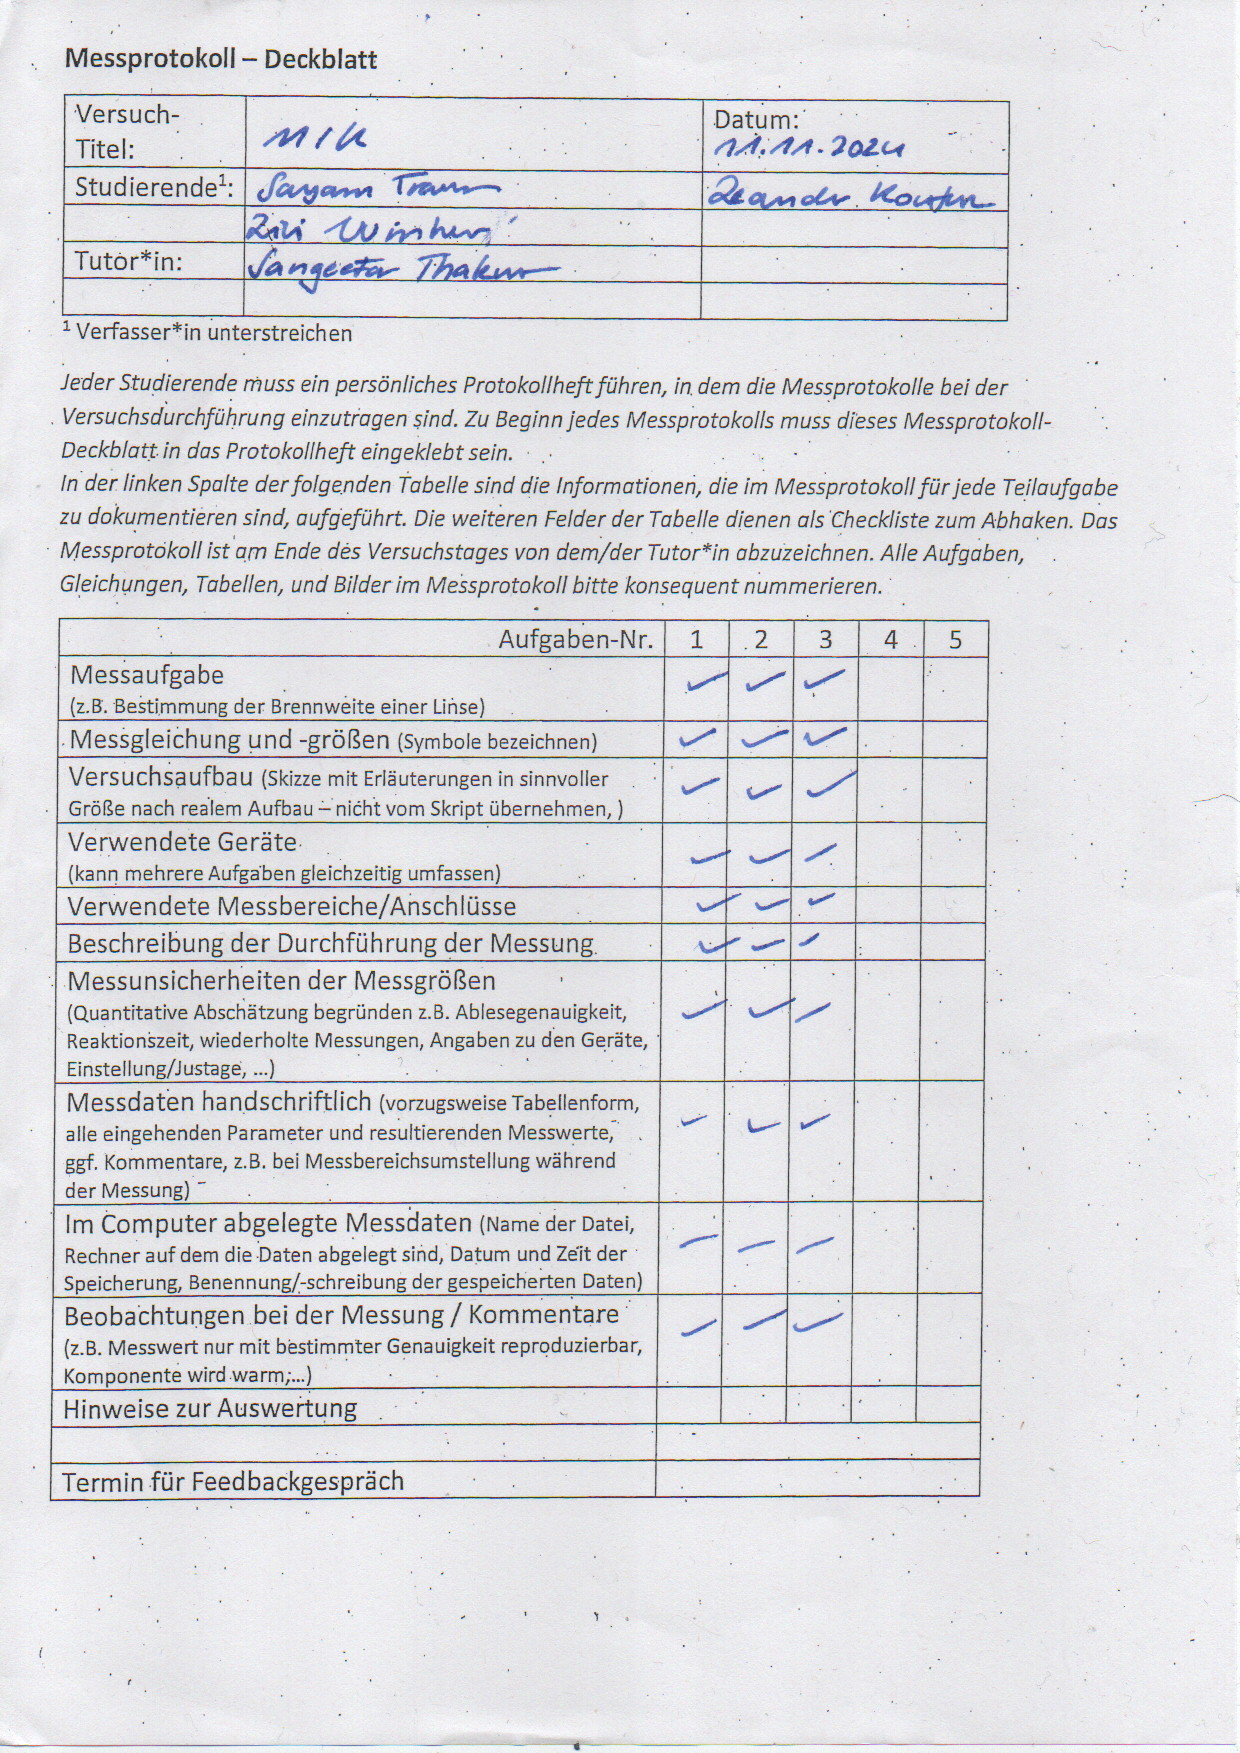
\includegraphics[scale=0.5]{Deckblatt_mik.jpg}
  \caption{Title page experiment MIK}
  \end{figure}


\begin{figure}[h!]
    \centering
  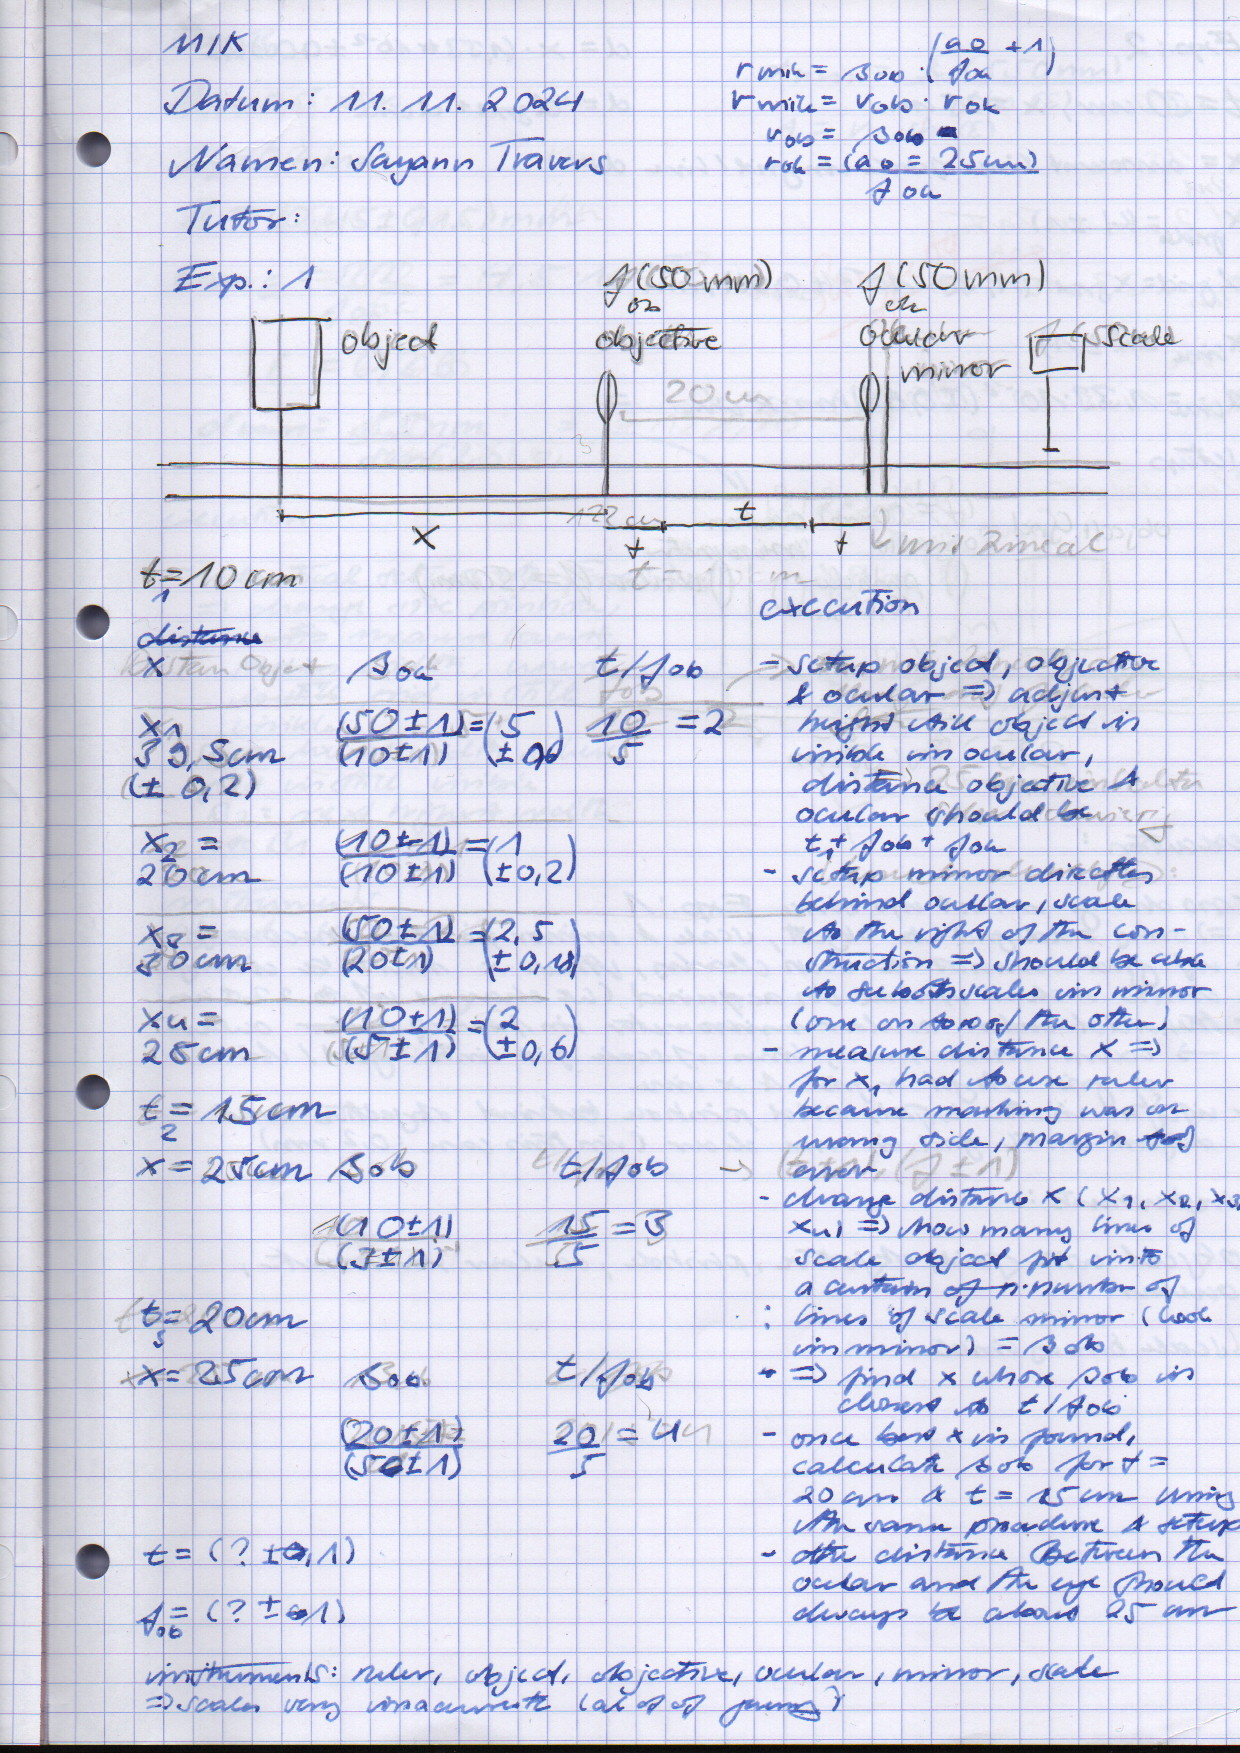
\includegraphics[scale=0.5]{Seite1_mik.jpg}
  \caption{Sayann Travers: Page 1 experiment MIK}
  \end{figure}


\begin{figure}[h!]
    \centering
  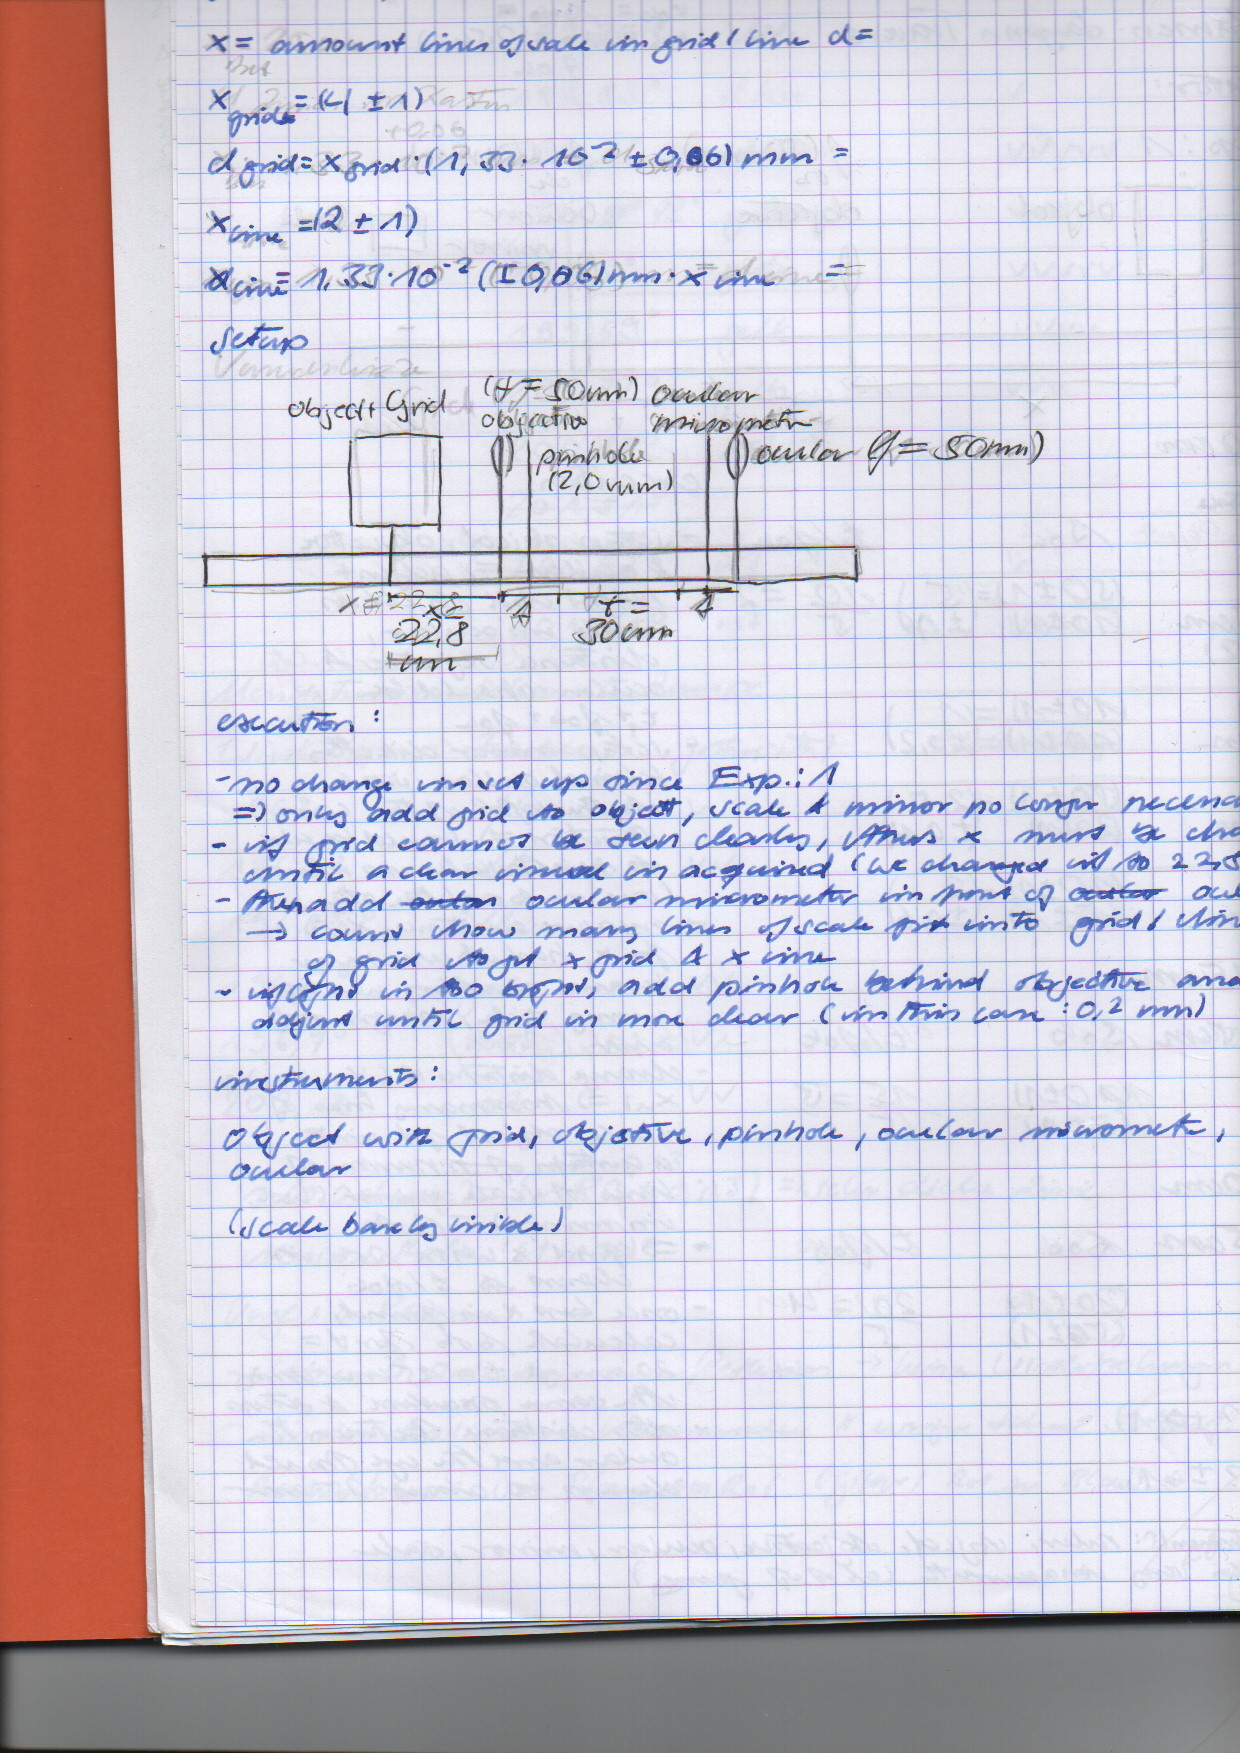
\includegraphics[scale=0.5]{Seite2_mik.jpg}
  \caption{Sayann Travers: Page 2 experiment MIK}
  \end{figure} 


\begin{figure}[h!]
    \centering
  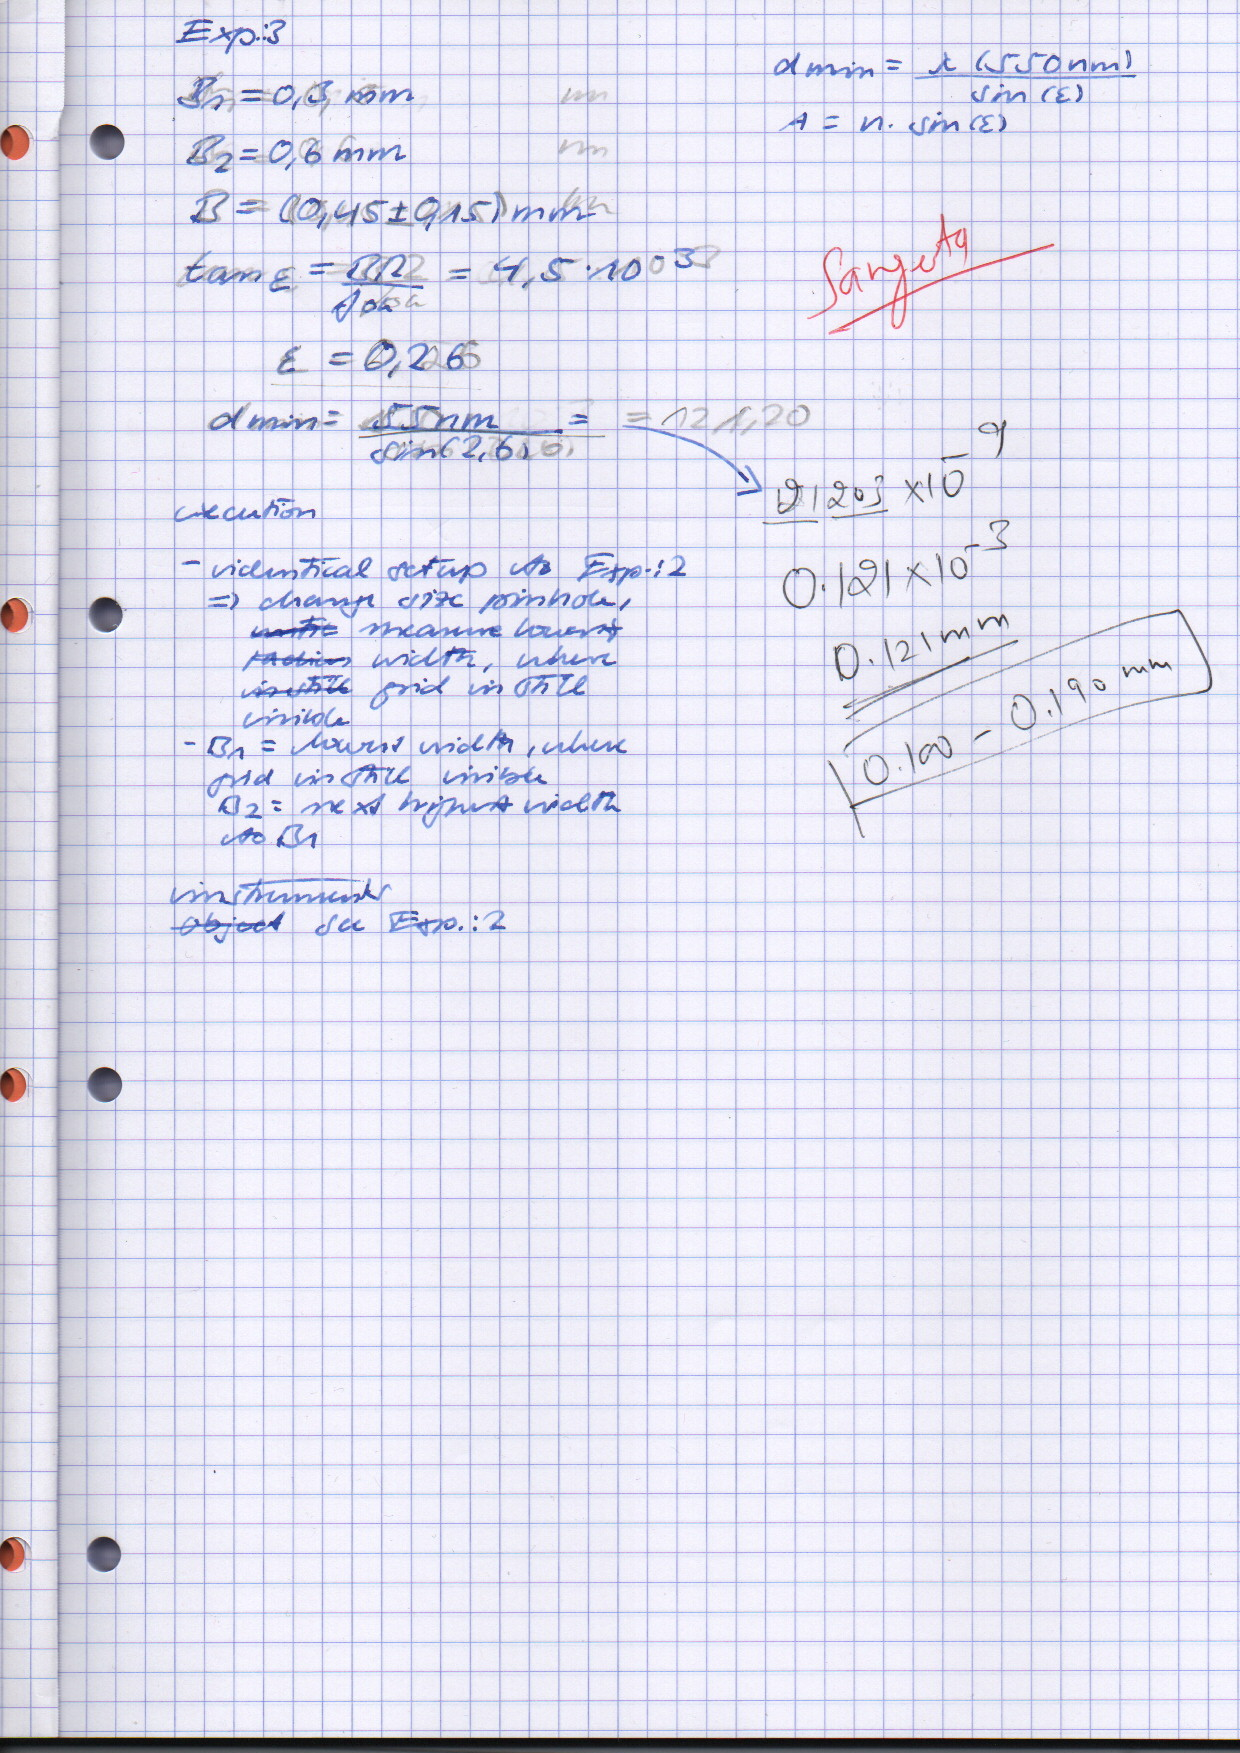
\includegraphics[scale=0.5]{Seite3_mik.jpg}
  \caption{Sayann Travers: Page 3 experiment MIK}
  \end{figure} 

\begin{figure}[h!]
    \centering
  \includegraphics[scale=0.5]{Dokument von Traveller.jpg}
  \caption{Leander Koufen: Experiment MIK}
  \end{figure} 



\end{document}
